\documentclass{article}

% Language setting
% Replace `english' with e.g. `spanish' to change the document language
\usepackage[english]{babel}
\usepackage{indentfirst}
% Set page size and margins
% Replace `letterpaper' with `a4paper' for UK/EU standard size
\usepackage[letterpaper,top=2cm,bottom=2cm,left=3cm,right=3cm,marginparwidth=1.75cm]{geometry}

% Useful packages
\usepackage{amsmath}
\usepackage{graphicx}
\usepackage[colorlinks=true, allcolors=blue]{hyperref}
\usepackage{float}%稳定图片位置
\usepackage{graphicx,subfig}%画图

\title{Entrepreneurship in Blockchain for Medicine: \\A Case Study in Plastic Surgery}
\author{Chongdan Pan}

\begin{document}
\maketitle

\begin{abstract}
Plastic surgery is a hot market that growing quite quickly with tens of millions of surgical procedures performed every year all over the world. However, at present, it's not a well-regulated industry as well since there are many cases that patients are injured or die from malpractice. The malpractice may be caused by the uncertificated doctor or unqualified medicine. The intransparency of the market has greatly increased the risk of taking plastic surgery. In this paper, we proposed a case study with a system built upon blockchain. The system stores the patients' data as well as all actions that the patients and doctors take as traceable and immutable records. The sensitive and private information will be encrypted so that only the owners can manage them, while other parts of the record can be used to identify how previous surgeries are performed. Thanks to the smart contract, the system can also facilitate the process of medical claims and transactions.
\end{abstract}
\section{Introduction}
Medicine is an area where multiple parties are involved. Patients, doctors, hospitals, and manufacturers are key stakeholders who interact with each other in a complex way. In these intricate flows, trust is extremely critical because misbehaving or false information may put people's lives at risk. The need for transparency and trust is more urgent in young and popular markets such as plastic surgery, where over 24 million surgical procedures were performed by more than 43750 surgeons in 2020\cite{ISAPS}. The market is large as well as chaotic, especially in some new markets like China. In 2019, the size of the medical aesthetics market in China amounted to 177 billion yuan, with a yearly growth of 22 percent \cite{ChinaMarket}. However, there were only less than 24\% licensed doctors, and less than 12\% regulated institutions\cite{ChinaReport}. To pursue a high profit, a large number of unqualified institutions and individuals are performing underground plastic surgeries without being regulated.
\par Underground plastic surgeries are risky in many aspects. The surgeon may be uncertificated and the medicine may not be approved for use in plastic surgery, which expose patients to malpractice. The outcomes of malpractice are serious, including infection, disfigurement, or even death. However, patients rarely pay attention to it due to the lack of information. Typically, people tend to rely on other customers' reviews for specific institutions or doctors, but it's unreliable due to false marketing. To solve this problem, this paper proposes a solution based on blockchain to track and transparentize surgery information. Our solution can authenticate customers' reviews and  previous activities for each surgeon and serve as a reliable platform where customers can find surgeons who most satisfy their needs.  
\par Blockchain was introduced to the world as the fundamental technology of Bitcoin by Satoshi Nakamoto in 2008\cite{Bitcoin}. Blockchain is designed to keep a record of every transaction in the Bitcoin system in a decentralized and immutable way. In the past few years, Bitcoin has resisted multiple network attacks and reached a total market value of over 500 billion USD, proving the reliability and robustness of blockchain technology. To interact with the blockchain, the user only needs to generate a random private key and public key pair like username and password for verification. Then, they can call the function deployed on the blockchain to make a transfer and their state like balance and call history will be recordede in blocks.
\par Our solution is a pubic decentralized application running on a blockchain and driven by smart contracts, "scripts that reside on the blockchain that allows for the automation of multi-step processes"\cite{SmartContract}. Compared to transaction record used in Bitcoin, smart contracts can be complexer and keep more information than a user's balance. For example, the smart contract can keep all surgeries and related information that a user has taken. The codes of smart contracts are open to the public so people can know the how the application run to every detail. Since blockchain will record all users' action and related data immutably, information like customer reviews and surgeons' previous activities are natually authenticated. Therefore, customers can track any information recorded on the blockchain and verify their authenticity. 
\par Besides building the trust between users, blockchain can be used to manage data as well. The loss from healthcare data breach is increasing rapidly in past a few years and people may be concerned that their private information is volunerable to cyber attack\cite{breach}. Thanks to decentralization and cryptography, this won't be an issued for blockchain. Since there's no single point failure in decentralizaed system, blockchain system is more resistent to database attack while teh cryptography ensured that only people with private key can be verified to manipulate the corresponding data.
\section{Existing Traditional Solution: Zocdoc}
Zocdoc is a streamlined system that provides patients with higher accessibility to doctors \cite{zocdoc}. When patients want to make a schedule with a doctor, the system can automatically provide a recommendation based on the patients' locations and other requirements. What's more, patients can publish their reviews for doctors on the application, which can be a good reference for other users. Then, patients and doctors can make an appointment for a further meeting. In plastic surgeries, the reviews can be extremely important for patients, because typically it's hard to know whether the doctor is certificated and how the surgery is conducted.
\par A common issue for Zocdoc is the reliability of the reviews. The doctor may post some fake reviews to raise the profile and attracts more customers. The phenomenon is very common in e-commerce platforms, where people can't trust the reviews anymore. Another major problem for Zocdoc is the patient may cancel or miss the appointment. As a result, the time of the clinic is lost and the revenue is decreased. Currently, Zocdoc will lock the patient's account if for multiple reschedules or cancellations, but the patient can avoid the side effect by setting up a new account. 
\par Compared to an open-source decentralized application running on the blockchain, people may be worried about the mechanism of the Zocdoc software system. On one hand, since all users' data are managed by the Zocdoc in a centralized way, there is a higher chance that the user's information is leaked in a data breach targeted to Zocdoc's database. On the other hand, users may be concerned about whether Zocdoc is giving them the best recommendation because doctors may pay a premium to Zocdoc for a higher recommendation rate. 
\par In conclusion, Zocdoc is trying to build trust between surgeons and patients and improve customers' experience. Although there are flaws within the existing system, Zocdoc's popularity has proven that there is a great demand for trust and convenience in the healthcare industry. However, the application is limited by the drawbacks in some aspects. For example, if the system recommends an uncertificated doctor to patients, Zocdoc's reputation will be badly affected. If patients are uncomfortable with how Zocdoc deals with their account, extra manual efforts or manual service is required as well.
\section{Our solution for Plastic Surgery Industry}
\subsection{Introduction}
To solve the problems in the plastic surgery industry and medicine accessibility, we designed a system built upon blockchain, to make the process more transparent, reliable, and smooth for patients to get service from plastic surgeons. The blockchain can not only be used to manage the patient's health data or claims but also their interactions with doctors, insurance companies, as well as medicine manufacturers. In this way, all actions and reviews are recorded on the blockchain so that patients can know how reliable the surgeon is by tracking the historical records. What's more, the blockchain can record important information about prescription medicine to make sure they're qualified and safe.
\par For now, a prototype has been developed by Solidity, a programming language specialized in designing smart contracts running on Ethereum Virtual Machine. After generating an identification key, patients can start by proposing a smart contract to a doctor's public address. The confidential information of a smart contract will be encrypted, but the status of each smart and the public key of users will be public. Depending on what status a smart contract is, people's behavior can be traced. If a patient misses an appointment, then the smart contract cannot proceed to the next stage. Since the users' public key and status of each smart are open to the public, the system can track how punctual the patient is. What's more, the smart contract ensures a seamless connection between data upload and payment. For example, the patient's medical history record will only be valid and stored on the blockchain when the user makes the necessary payment.
\subsection{Actors}
\subsubsection{Doctors}
Doctors are using the system to promote themselves and attract customers so that they can get greater revenue. To get certificated and attractable for patients, the doctor needs to make important information public on the system, including digital identity and license. Since the license number is traceable, we can check whether the doctor is using a verified license or a fake one. The digital identity is like the public address or public key of the doctor. Knowing the doctor's public key, patients can either propose a smart contract to request an appointment or trace the doctor's previous activities on the blockchain. In addition, the patient can use the doctor's public key to encrypt the sensitive medical records and send them to the doctor. The transmission of the medical records will be recorded publicly on the blockchain, but its sensitive content is secure and only visible to the doctor thanks to the property of asymmetric encryption\cite{encryption}. The digital identity will be recorded on the blockchain with all actions that the doctor made, such as surgeries, prescriptions, examinations, and the review that the doctor got. Although the sensitive information in these actions is encrypted, people can still evaluate a doctor based on historical records and reviews.
\subsubsection{Patients}
Patients are other primary users of the system. The blockchain enables them to manage their data safely, as well as find reliable doctors based on the historical information stored on the blockchain. Before entering the system, the user needs to generate a public-private key pair. After the doctors' office visit, the doctor will use the public key to encrypt the patient's new medical history records and store them on the blockchain. In this way, only the patients and the doctor who uploaded the records can see the sensitive content. For doctors, they won't have any incentive to leak the information because people can easily check who may view the information and such action can injure the reputation. Hence, the patients have full control of the medical history records since nobody can see them later without the patient's private key. The patient's public key can be used to identify the patient as well since it represents the owners of the medical history records. Therefore, doctors can check the miss and reschedule rate of a patient as well be searching for the patient's historical actions on the blockchain.
\subsubsection{Third Parties}
Third parties can be other stakeholders or people who have an interest in the system, such as medicine manufacturers and insurance companies. A lot of plastic surgery malpractice is due to unqualified medicine, hence manufacturers will be asked to upload the serial number of medicine used in each prescription to the blockchain so that they can be verified and traceable. Storing the medicine information on the blockchain can also help the medicine manufacturers to manage the supply chain efficiently. For insurance companies, they can inject the insurance terms into the smart contract set between patients and doctors. With the help of a smart contract, the insurance can be more clearly identified and executed as automatically as possible.
\subsection{Workflow}
\begin{figure}[H]
    \centering
    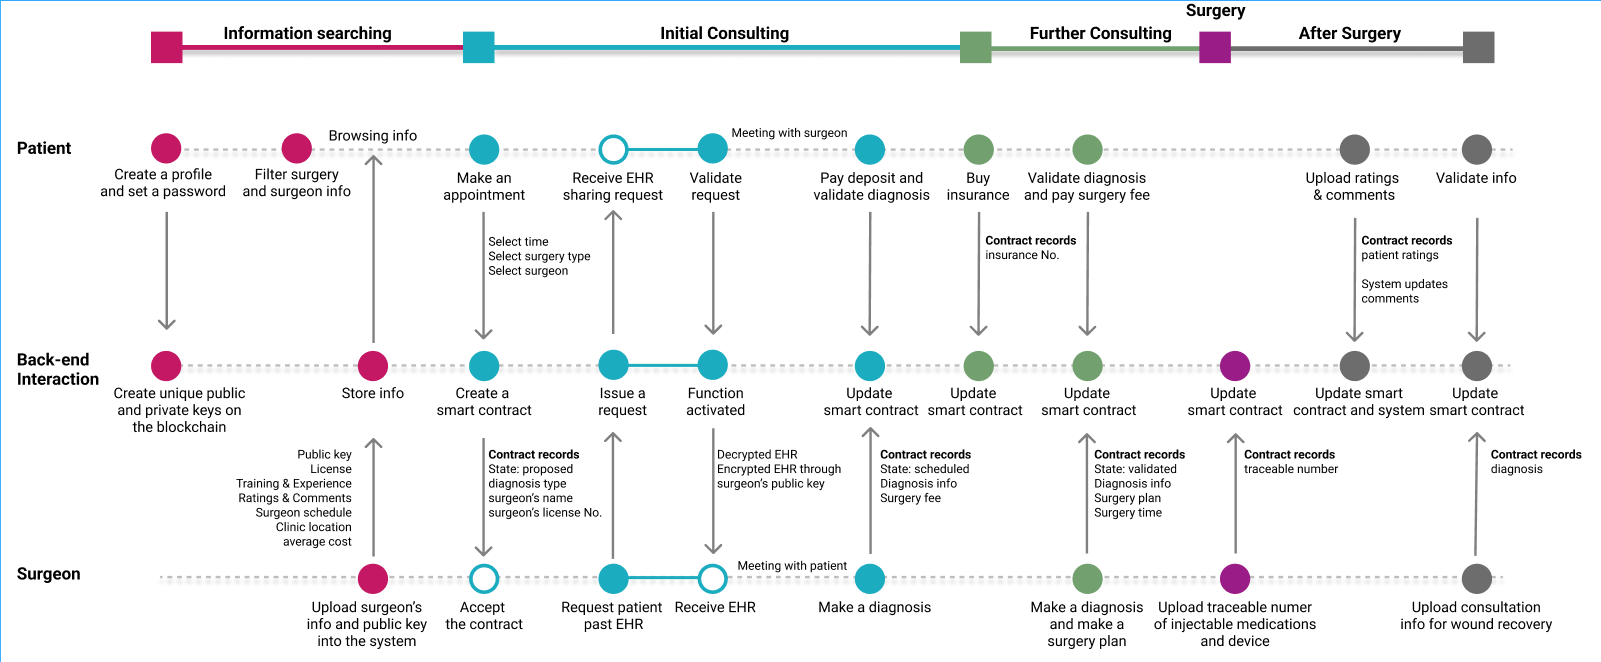
\includegraphics[scale=0.45]{Workflow.jpg}
    \caption{Example of our solution's work flow}
\end{figure}
The workflow between patients and doctors based on our system can be divided into four stages.
\subsubsection{Information Searching}
In this initial stage, patients and doctors need to create their private-public key pair so that the patient can set up a secure account to store health data and the doctor can become searchable. Then, the patient can search for doctors based on the initial public information stored on the blockchain.
\begin{figure}[H]
    \centering
    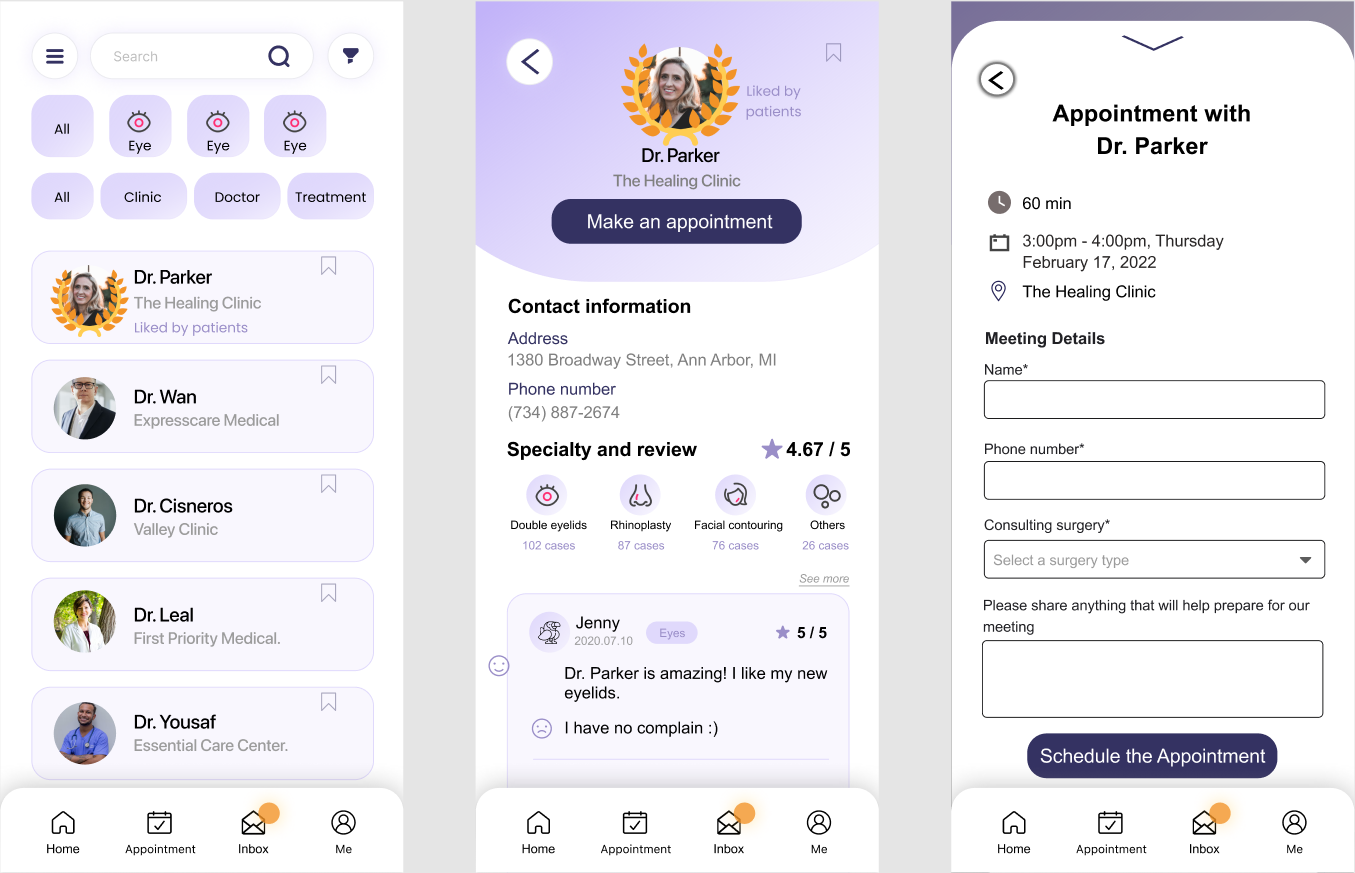
\includegraphics[scale=0.5]{Appointment.jpg}
    \caption{Information Search}
\end{figure}
The searching process is very similar to the existing application, and then the patient can propose a smart contract with an appointment time to the doctor's public address. The creation of a smart contract will cause some transaction fees since it needs to store new data on the blockchain. During the searching process, previous patients' reviews can serve as a reference. Users can make choices either based on the previous review or the smart contract records associated with a specific doctor. Different from the traditional system, it's impossible for the doctor to fake the review because they're linked to a  smart contract containing all immutable information regarding the treatment. If the doctor wants to make a fake review, he or she must go through the whole process from proposing a smart contract to the end of visiting, which requires a lot of time and money.
\subsubsection{Initial Consulting}
If the doctor accepted the smart contract by putting a digital signature on it, all basic information of patients and patients will be stored with it. Then the doctor can send a request for the patient's previous medical history record. Once received the request, only the patient who has the private key can determine whether to share it, because the medical history record is stored on the blockchain encrypted by the patient's key. If the patient authorizes the access, the records will be decrypted by the patient's key and encrypted by the doctors' key again so that only the doctor can view it.
\begin{figure}[H]
    \centering
    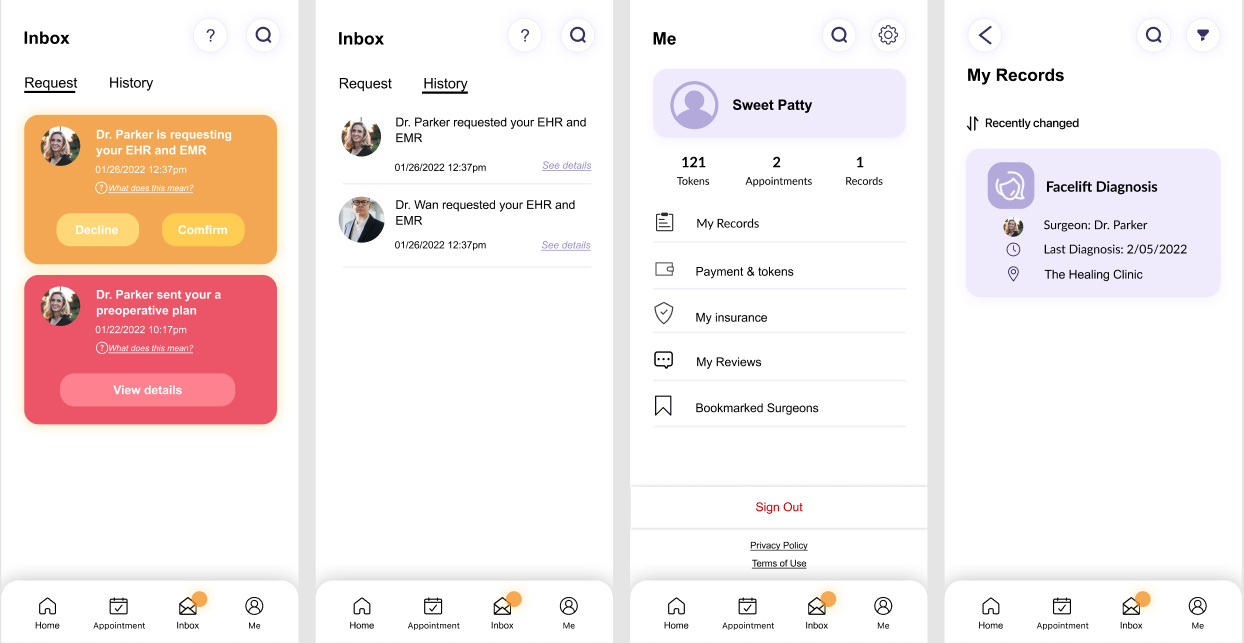
\includegraphics[scale=0.5]{InitialConsulting.jpg}
    \caption{Initial Consulting}
\end{figure}
\subsubsection{Further Consulting}
After the first consultation, doctors and patients should have a plan for the following surgery. In this stage, the smart contact can be linked to the insurance claims with clear terms. In this stage, the patient also needs to confirm the surgery plan by paying the deposit for it.
\begin{figure}[H]
    \centering
    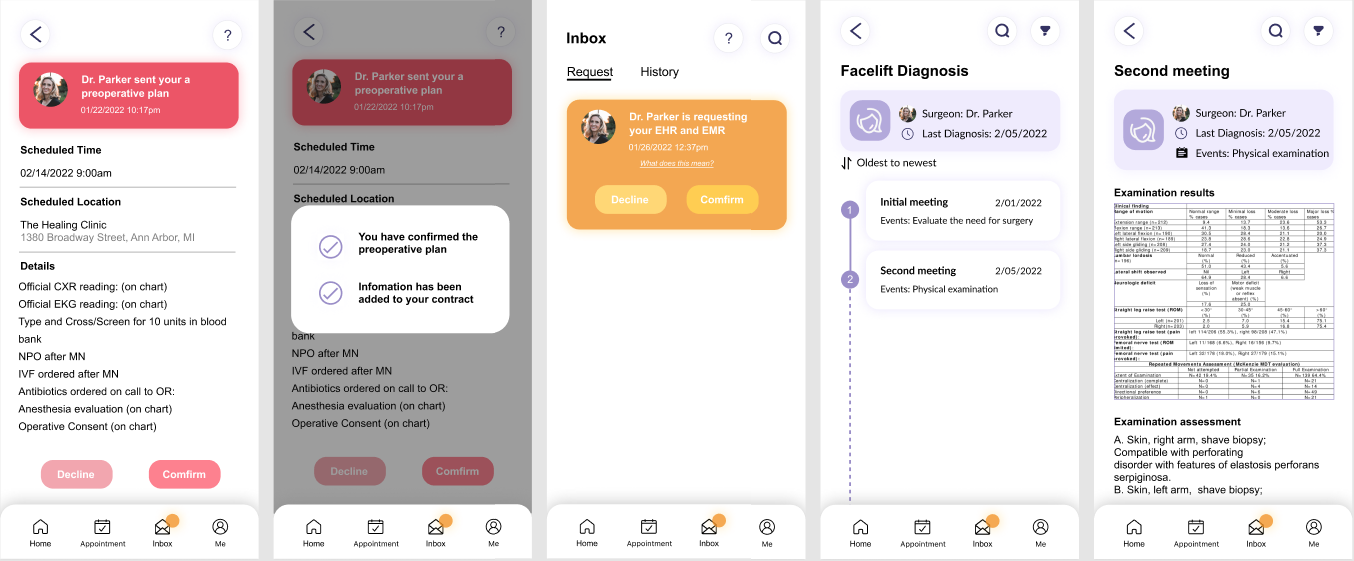
\includegraphics[scale=0.5]{SecondConsulting.jpg}
    \caption{Information Search}
\end{figure}
The surgery can proceed only after all previous diagnoses are verified and both the doctors and patients agree on the plan. All other medicine used in the surgery, such as anesthetics, should be recorded on the blockchain as well. Since everything is confirmed and recorded clearly, it'll be easy to track if there is something that happens with the surgery. 
\subsubsection{After surgery}
After the surgery, the doctor will encrypt the surgery summary and further prescription with the user's public key and upload the data on the blockchain. The smart contract will make sure that the data will only be valid after the user's confirmation and complete the transaction. The surgery summary will be designed to be structured so it can match well with the insurance term. If it matches any term, the smart contract will automatically execute it and proceed with the health claims.
\par When the patient's medical health records are validated, they will be encrypted and linked to the patient's public key, so that the patient can manage it later. In addition, the patient will be incentivized to provide a review for the doctor to help other patients make a choice.
\subsection{Challenges}
A major challenge for this system is how to be docked to the current medical system. Lots of people have their medical history records stored in the traditional system right now, and it'll take huge efforts to encrypt and upload them on the blockchain. The complexity of blockchain may also hinder users from using our system.
\par In the technology aspect, the system is designed to be running on a blockchain using Algorand consensus, which is claimed to be able to solve the blockchain trilemma with high scalability\cite{algorand}. However, due to the rapid development of blockchain technology, we think it will be helpful to set up a middle layer between our application with the layer-one solution like a virtual machine. In this way, the application and data can be easily transferred to a more advanced blockchain.
\par The volatility of blockchain tokens can be a challenge. Patients hope the cost for a surgery won't fluctuate all over time so that they can make a budget plan while the doctors want to get stable revenue. Since users of blockchain can't directly make payments through fiat currency, they need some way to make an exchange. One way to reduce volatility is to use stable tokens, but it also poses a challenge to control the issue of the token.
\par The complexity of smart contracts will make it challenging to set a standard way for it to proceed. Patients and doctors may have a disagreement on the status of a smart contract or what information should be considered as sensitive and need to be encrypted. The smart contract may lead to other problems that are hard to be solved by the law.
\section{Conclusion}
In this paper, we have an overview of the current plastic surgery industry and identify some problems and some existing solutions. Then we present a system built upon blockchain to make the industry more transparent, trustworthy, and efficient than ever. The immutability and traceability of the blockchain system make sure that everyone's action is recorded publicly so that patients can find reliable doctors and medicine based on previous records. Thanks to cryptography, the system also ensures the security of patient's private data. The smart contract makes the transaction between patients and doctors smoother and enables the automatic execution of insurance claims. The system is designed to reduce the requirement of trust between users and make the process automatically as much as possible. It's fully viable since it can be built upon existing technology. 
\bibliographystyle{plain}
\bibliography{Reference}

\end{document}